\chapter{Produktprincip}
Produktets vil være en webapp løsning, som ved brug af Googles bruger API og fragtfirma 
api’er såsom GLS’s og Postnords API'er. skal kunne gennemsøge den brugerens gmail og 
derudfra hente trackingnummer på forsendelser fra en bred vifte af fragtfirmaer. denne 
tracking information skal derefter fremvises til brugeren på webappen, således tracking 
informationen fra alle brugerens pakker samles.
\section{Flowchart over programmet}
\begin{figure}[h]
    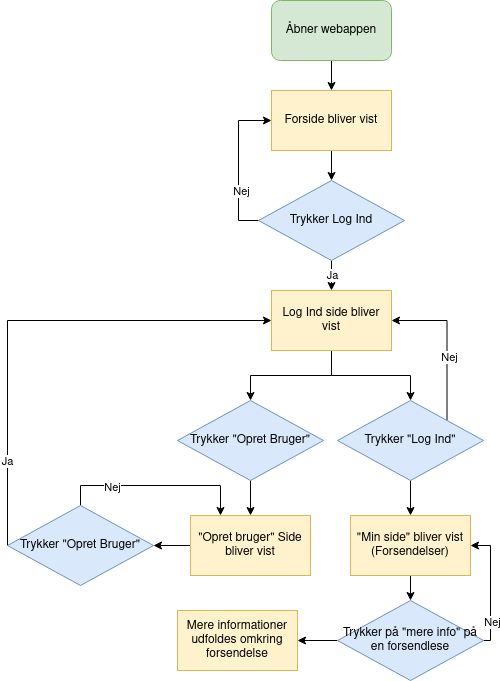
\includegraphics[width=0.5\linewidth]{Pictures/flowchat-main.png}
    \centering
    \caption{General funktion af programmet.}
     \label{fig:drill-backplate}
  \end{figure}
  

\section{Produktkrav}
Der er her opstillet en række hårde og bløde krav som det udviklede web app skal opnå. de er som følger:

Hårde krav:
Skal kunne tracke pakker fra mindst 2 forskellige fragtfirmaer
Skal kunne fremvise pakke tracking fra mindst 2 forskellige fragtfirmaer det samme sted
Oprette bruger
siden skal have en lav kompleksitet (tilgå tracking på 2 klik)

Bløde Krav:
Skal have et moderne stilrent design
Oprette bruger med Google
Skal fungere upåklageligt på mobile enheder (være responsivt)
Skal selv kunne hente mails fra brugerens google konto
